\input{../../.preambles/01-semester_work}
\input{../../.preambles/10-russian}
\input{../../.preambles/20-math}
\input{../../.preambles/22-vectors}
\input{../../.preambles/30-physics}
\usepackage{wrapfig}

\begin{document}
\maketitlepage{Факультет электроники и вычислительной техники}{физики}
{Электродинамика}{3}{}{студент группы Ф-369\\Голубев~А.~В.}
{}{доцент Грецов~М.~В.}{}{}

\emph{Задача №1.15}: Определить поле, создаваемое заряженным проводящим шаром 
радиуса \( a \). Заряд его \( Q \). Диэлектрическая проницаемость окружающей 
среды \( \eps = \eps(r) \), где \( r \) -- расстояние от центра шара.

\emph{Решение:} 

\begin{wrapfigure}[10]{l}{0.4\textwidth}
	\vspace{-2ex}
	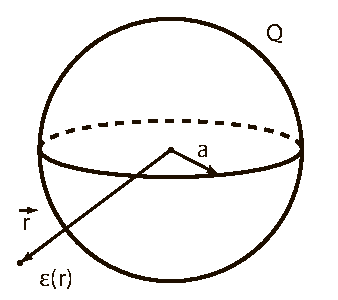
\includegraphics[width=0.4\textwidth]{pdf/image_1_15}
\end{wrapfigure}

Для решения задачи воспользуемся сферической системой координат. Учтём, что 
задача имеет сферическую симметрию и запишем следующие соотношения:
\[
	D_r = D(r);\quad
	D_\theta = D_\psi = 0
\]

Электрическая индукция поля может быть записана в следующем виде:
\[
	\div{\vec{D}} = \rho
\]

Воспользуемся теоремой Остроградского-Гаусса, перепишем предыдущее равенство 
в виде:
\[
	\int \div\vec{D} dV = \oint \vec{D}\vec{dS} = \int \rho dV = q
\]

Перепишем предыдущее в виде:
\[
	D \oint\vec{dS} = DS = q
\]

Поле внутри шара (\( r < a, q = 0 \)):
\[
	D = E = 0
\]

Поле вне шара (\( r > r, q = Q \)):
\[
	D = \frac{Q}{4\pi r^2}
\]

C учётом \( D = \eps_0\eps E \), получим:
\[
	E = \frac{Q}{4\pi\eps_0\eps(r) r^2}
\]

\emph{Ответ:} \( D = \cfrac{Q}{4\pi r^2},\quad E = \cfrac{Q}{4\pi\eps_0\eps(r) r^2}\)
 
\newpage

\emph{Задача №1.58}: Вычислить ёмкость цилиндрического конденсатора. Длина 
его \( l \), радиусы обкладок \( R_1 \) и \( R_2 \). Между обкладками два 
коаксиальных слоя однородных диэлектриков с проницаемостями \( \eps_1 \) 
и \( \eps_2 \), граница раздела между ними -- цилиндрическая поверхность 
радиуса \( R_0 \). Краевыми эффектами пренебречь.

\emph{Решение:}

\begin{wrapfigure}[10]{l}{0.4\textwidth}
	\vspace{-2ex}
	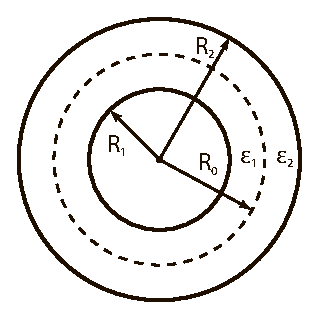
\includegraphics[width=0.4\textwidth]{pdf/image_1_58}
\end{wrapfigure}

Вычислим поле между обкладками конденсатора с проницаемостью \( \eps \), 
высотой \( l \) и зарядов \( q \). 

Начнём поиск поля в точке \( r \) находящегося между обкладками. Используя 
теорему Гаусса, с учётом соноправленности векторов \( S \) и 
\( dS \), получим:
\[ 
	\oint\limits_S \vec{E}\vec{dS} = \oint\limits_S EdS = 
	E \oint dS = E \cdot 2\pi r l = \frac{q}{\eps\eps_0}
\]
\[
	E(r) = \frac{q}{2\pi\eps\eps_0 rl}
\]

Тогда напряженность поля между обкладками будет:
\[
	E(R) = \frac{q}{2\pi\eps\eps_o Rl}
\]

Отсюда находим разность потенциалов:
\[
	\phi_1 - \phi_2 = \int\limits^{R_2}_{R_1} E(R) dR = 
	\frac{q}{\eps_0 l} \left( 
		\int \limits^{R_0}_{R_1} \frac{1}{\eps_1 R} + 
		\int \limits^{R_2}_{R_0} \frac{1}{\eps_2 R} 
	\right) = 
	\frac{q}{\eps_0 l} \left(
		\frac{1}{\eps_1}\ln\frac{R_0}{R_1} + 
		\frac{1}{\eps_2}\ln\frac{R_2}{R_0}
	\right) 
\]

Тогда ёмкость:
\[
	C = \frac{q}{\phi_1 - \phi_2} = 
	\frac{l}{ \cfrac{1}{\eps_1}\ln\cfrac{R_0}{R_1} + 
	\cfrac{1}{\eps_2}\ln\cfrac{R_2}{R_0}}
\]

\emph{Ответ:} \(
	C = \cfrac{q}{\phi_1 - \phi_2} = 
	\cfrac{l}{ \cfrac{1}{\eps_1}\ln\cfrac{R_0}{R_1} + 
	\cfrac{1}{\eps_2}\ln\cfrac{R_2}{R_0}}
\)

\newpage

\emph{Задача №1.99}: Точечный заряд \( q \) находится на одинаковом 
расстоянии \( a \) от двух взаимно перпендикулярных заземленных проводящих 
полуплоскостей. Определить создаваемое поле.

\emph{Решение:}

\begin{wrapfigure}[10]{l}{0.4\textwidth}
	\vspace{-5ex}
	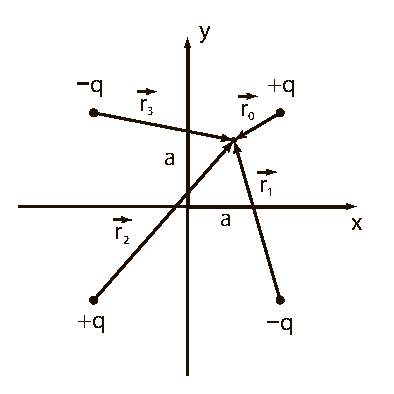
\includegraphics[width=0.4\textwidth]{pdf/image_1_99}
\end{wrapfigure}

Выберем положение полуплоскостей как показано на рисунке. Начало отсчёта 
в точке пересечения полуплоскостей. Воспользуемся методом изображений 
построим изображение заряда. 

Найдём потенциал в произвольной точке системы:
\[ 
	\phi = \frac{q}{4\pi\eps_0}\left( \frac{1}{r_0} - \frac{1}{r_1} + 
	\frac{1}{r_2} - \frac{1}{r_3} \right) 
\] 
где \( r_0 \) -- расстояние рассматриваемой точки поля от заряда \( q \), а 
\( r_1, r_2, r_3 \) -- от его изображений.
\[
	r_0 = \sqrt{(x-a)^2 + (y-a)^2 + z^2};\quad
	r_1 = \sqrt{(x-a)^2 + (y+a)^2 + z^2}
\]
\[
	r_2 = \sqrt{(x+a)^2 + (y+a)^2 + z^2};\quad
	r_3 = \sqrt{(x+a)^2 + (y-a)^2 + z^2}
\]

Подставляя в потенциал получаем:
\begin{equation*}
\begin{split}
	\phi = \frac{q}{4\pi\eps_0}\Big(
		\frac{1}{\sqrt{(x-a)^2 + (y-a)^2 + z^2}} - 
		\frac{1}{\sqrt{(x-a)^2 + (y+a)^2 + z^2}} + \\ +
		\frac{1}{\sqrt{(x+a)^2 + (y+a)^2 + z^2}} -
		\frac{1}{\sqrt{(x+a)^2 + (y-a)^2 + z^2}}
	\Big)
\end{split}
\end{equation*}

Поле создаваемое зарядом:
\[ E = -\grad\phi \]

Подставляя значение потенциала получаем:
\[
	E = -\frac{q}{4\pi\eps_0}\left\{
		\frac{d\Phi}{dx}, 
		\frac{d\Phi}{dy}, 
		\frac{d\Phi}{dz}
	\right\} \text{, где}
\]
\begin{equation*}
\begin{split}
	\frac{d\Phi}{dx} = \frac{x-a}{\left( (x-a)^2 + (y-a)^2 + z^2\right)^{\frac{3}{2}}} -
	\frac{x-a}{\left( (x-a)^2 + (y+a)^2 + z^2\right)^{\frac{3}{2}}} + \\ + 
	\frac{x+a}{\left( (x+a)^2 + (y+a)^2 + z^2\right)^{\frac{3}{2}}} -
	\frac{x+a}{\left( (x+a)^2 + (y-a)^2 + z^2\right)^{\frac{3}{2}}} \\
	\frac{d\Phi}{dy} = \frac{y-a}{\left( (x-a)^2 + (y-a)^2 + z^2\right)^{\frac{3}{2}}} -
	\frac{y+a}{\left( (x-a)^2 + (y+a)^2 + z^2\right)^{\frac{3}{2}}} + \\ + 
	\frac{y+a}{\left( (x+a)^2 + (y+a)^2 + z^2\right)^{\frac{3}{2}}} -
	\frac{y-a}{\left( (x+a)^2 + (y-a)^2 + z^2\right)^{\frac{3}{2}}} \\
	\frac{d\Phi}{dz} = \frac{2z}{\left( (x-a)^2 + (y-a)^2 + z^2\right)^{\frac{3}{2}}} -
	\frac{2z}{\left( (x-a)^2 + (y+a)^2 + z^2\right)^{\frac{3}{2}}} + \\ + 
	\frac{2z}{\left( (x+a)^2 + (y+a)^2 + z^2\right)^{\frac{3}{2}}} -
	\frac{2z}{\left( (x+a)^2 + (y-a)^2 + z^2\right)^{\frac{3}{2}}} \\
\end{split}
\end{equation*}

\newpage

\emph{Задача №2.35}: Полупространство заполнено однородным магнетиком с 
проницаемостью \( \mu_1 \), а второе полупространство -- однородным 
магнетиком с проницаемостью \( \mu_2 \). В первой среде имеется плоский 
контур \( L \) с током \( I \), расположенный параллельно плоскости 
раздела обеих сред на расстоянии \( h \) от неё. Определить создаваемое 
током магнитное поле.

\emph{Решение:}

\begin{wrapfigure}[10]{l}{0.4\textwidth}
	\vspace{-2ex}
	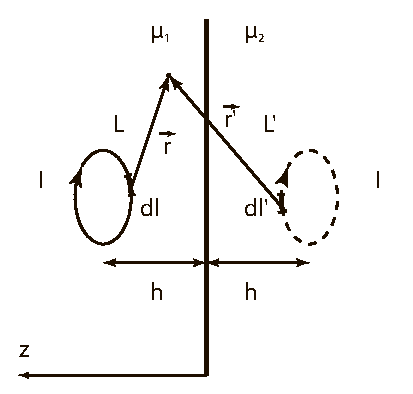
\includegraphics[width=0.4\textwidth]{pdf/image_2_35}
\end{wrapfigure}

Выберем плоскость раздела двух сред за координатную (\( z = 0 \)) и направим в 
сторону первой среды.

Вектор-потенциал искомого поля будем искать в виде:
\[
	\vec{A}_1 = \frac{\mu_1 I}{c} \oint \frac{d\vec{l}}{r} + 
		\frac{\mu_1 k_1 I}{c} \oint \frac{d\vec{l'}}{r'} \eqno{1}
\]
\[
	\vec{A}_2 = \frac{\mu_2 k_2 I}{c} \oint \frac{d\vec{l}}{r} \eqno{2}
\]

где \( l' \) -- изображение контура \( l \), \( r \) и \( r' \) -- 
расстояние рассматриваемой точки поля от элемента длины \( dl \) и \( dl' \).

\begin{wrapfigure}[8]{l}{0.4\textwidth}
	\vspace{-5ex}
	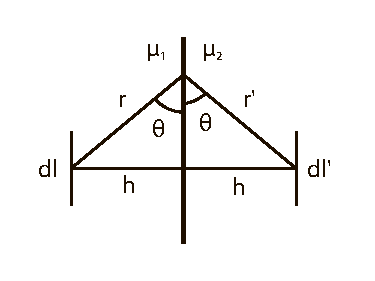
\includegraphics[width=0.4\textwidth]{pdf/image_2_35_2}
\end{wrapfigure}

Рассмотрим условие непрерывности векторного потенциала на границе
двух сред, где 
\[ A_1 = A_2 \eqno{3}\]
тогда:
\[
	r = hcos\theta;\quad r' = hcos\theta
\]

Подставляя \( (1) \) и \( (2) \) в уравнение \( (3) \) получаем:
\[
	\frac{\mu_1 I}{ch\cos\theta} \oint dl + 
	\frac{\mu_1 k_1 I}{ch\cos\theta} \oint dl' = 
	\frac{\mu_2 I}{ch\cos\theta} \oint dl
\]

В силу произвольности элемента \( dl \) и \( dl' \):
\[ 
	\left( 1 + k_2 \right) \mu_1 + \mu_2 k_1 = 0
\]

Рассмотрим непрерывность производной на границе:
\[
	\frac{1}{\mu_1}\pder{A_1}{n} + \frac{1}{\mu_2}\pder{A_2}{n} = \frac{I}{c}
\]

\pagebreak

Подставляя уравнения для потенциалов и учитывая произвольность элементов 
\( dl \) и \( dl' \) получаем:
\[
	k_1 + k_2 = 1
\]

С учётом предыдущей формулы связывающие \( k_1 \) и \( k_2 \) получаем:
\[
	k_1 = \frac{\mu_2 - \mu_1}{\mu_2 + \mu_1};\quad
	k_2 = \frac{2\mu_1}{\mu_1 + \mu_2}
\]

Подставляя в векторный потенциал получаем:
\[
	\vec{A}_1 = \frac{\mu_1 I}{c} \oint \frac{d\vec{l}}{r} + 
		\left(\frac{\mu_2 - \mu_1}{\mu_2 + \mu_1}\right)
		\frac{\mu_1 I}{c} \oint \frac{d\vec{l'}}{r'}
\]
\[
	\vec{A}_2 = \left(\frac{2\mu_1}{\mu_1 + \mu_2}\right)
	\frac{\mu_2 I}{c} \oint \frac{d\vec{l}}{r}
\]

Тогда поле создаваемое плоским контуром в произвольной точке будет:
\[
	\vec{B} = \rot\vec{A}_1 + \rot\vec{A}_2
\]
\[
	\vec{H} = \frac{1}{\mu_1}\rot\vec{A}_1 + \frac{1}{\mu_2}\rot\vec{A}_2 
\]

\end{document}